\documentclass[12pt]{article}
\usepackage[utf8]{inputenc}
\usepackage{float}
\usepackage{amsmath}
\usepackage{tikz}
\usetikzlibrary{arrows,automata,positioning}
\usepackage{wrapfig, lipsum}
\usepackage{array}
\usepackage[hmargin=3cm,vmargin=6.0cm]{geometry}
\topmargin=-2cm
\addtolength{\textheight}{6.5cm}
\addtolength{\textwidth}{2.0cm}
\setlength{\oddsidemargin}{0.0cm}
\setlength{\evensidemargin}{0.0cm}
\usepackage{indentfirst}
\usepackage{amsfonts}
\usepackage[linguistics]{forest}

\begin{document}

\section*{Student Information}

Name : Emre Geçit\\

ID : 2521581\\


\section*{Answer 1}
\subsection*{a)} 
$((a\cup b)^*aa(a\cup b)^*bb(a\cup b)^*)\cup((a\cup b)^*bb(a\cup b)^*aa(a\cup b)^*)$
\begin{wrapfigure}{r}{0.57\textwidth}

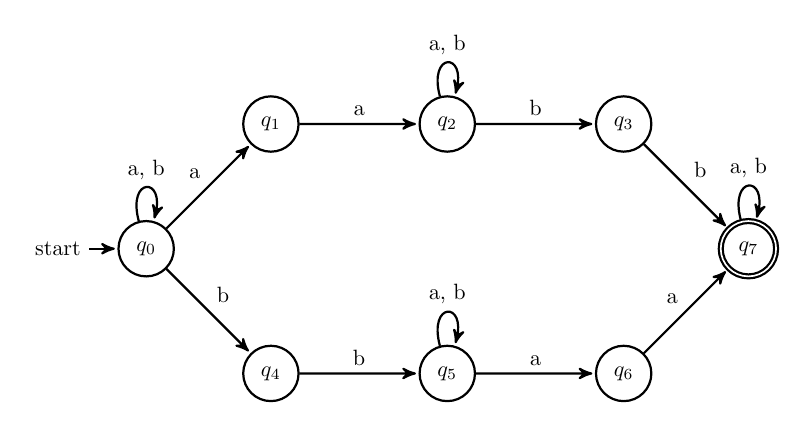
\begin{tikzpicture}[->,>=stealth',shorten >=1pt,auto,node distance=2.8cm,
                    thick, scale=0.8, every node/.style={scale=0.8}]
  \tikzstyle{every state}=[fill=white,draw=black,text=black]

  \node[initial,state] (q_0)                    {$q_0$};
  \node[state]         (q_1) [above right of=q_0] {$q_1$};
  \node[state]         (q_2) [right of=q_1] {$q_2$};
  \node[state]         (q_3) [right of=q_2] {$q_3$};
  \node[state]         (q_4) [below right of=q_0]       {$q_4$};
  \node[state]         (q_5) [right of=q_4] {$q_5$};
  \node[state]         (q_6) [right of=q_5] {$q_6$};
  \node[state, accepting]         (q_7) [below right of=q_3]       {$q_7$};

  \path (q_0) edge              node {a} (q_1)
            edge [loop above] node {a, b} (q_0)
            edge node {b} (q_4)
        (q_1) edge node {a} (q_2)
        (q_2) edge [loop above] node {a, b} (q_2)
            edge              node {b} (q_3)
        (q_3) edge node {b} (q_7)
        (q_4) edge node {b} (q_5)
        (q_5) edge [loop above] node {a, b} (q_5)
        (q_5) edge node {a} (q_6)
        (q_6) edge node {a} (q_7)

        (q_7) edge [loop above] node {a, b} (q_7)
        ;
\end{tikzpicture}
\end{wrapfigure}
\subsection*{b)}

Q = $\{q_0, q_1, q_2, q_3, q_4, q_5, q_6, q_7\}$

$\Sigma = \{a, b\}$

$s = q_0$

$F = \{q_7\}$

$\Delta$)
\begin{tabular}{ l l l } 
  \hline
  states & a & b \\ 
  \hline
  $q_0$ & $\{q_0, q_1\}$ & $\{q_0, q_4\}$ \\ 
  $q_1$ & $\{q_2\}$ & $\{\}$ \\
  $q_2$ & $\{q_2\}$ & $\{q_2, q_3\}$ \\
  $q_3$ & $\{\}$ & $\{q7\}$ \\
  $q_4$ & $\{\}$ & $\{q_5\}$ \\
  $q_5$ & $\{q_5, q_6\}$ & $\{q_5\}$ \\
  $q_6$ & $\{q_7\}$ & $\{\}$ \\
  $q_7$ & $\{q_7\}$ & $\{q_7\}$ \\
  \hline
\end{tabular}
\subsection*{c)}
\begin{tabular}{ l l l l}
  \hline
  states & a & b \\ 
  \hline
  $\{q_0\}$ & $\{q_0,q_1\}$ & $\{q_0,q_4\}$ & $\{q_0,q_1\}$, $\{q_0,q_4\}$ added\\
  $\{q_0,q_1\}$ & $\{q_0,q_1,q_2\}$ & $\{q_0,q_4\}$ & $\{q_0,q_1,q_2\}$ added\\
  $\{q_0,q_4\}$ & $\{q_0,q_1\}$ & $\{q_0,q_4,q_5\}$ & $\{q_0,q_4,q_5\}$ added\\
  $\{q_0,q_1,q_2\}$ & $\{q_0,q_1,q_2\}$ & $\{q_0,q_2,q_3,q_4\}$ & $\{q_0,q_2,q_3,q_4\}$ added\\
  $\{q_0,q_4,q_5\}$ & $\{q_0,q_1,q_5,q_6\}$ & $\{q_0,q_4,q_5\}$ & $\{q_0,q_1,q_5,q_6$\} added\\
  $\{q_0,q_2,q_3,q_4\}$ & $\{q_0,q_1,q_2\}$ & $\{q_0,q_2,q_3,q_4,q_5,q_7\}$ & $\{q_0,q_2,q_3,q_4,q_5,q_7\}$ added\\
  $\{q_0,q_1,q_5,q_6\}$ & $\{q_0,q_1,q_2,q_5,q_6,q_7\}$ & $\{q_0,q_4,q_5\}$ & $\{q_0,q_1,q_2,q_5,q_6,q_7\}$ added\\
  $\{q_0,q_2,q_3,q_4,q_5,q_7\}$ & $\{q_0,q_1,q_2,q_5,q_6,q_7\}$ & $\{q_0,q_2,q_3,q_4,q_5,q_7\}$ & no new state\\
  $\{q_0,q_1,q_2,q_5,q_6,q_7\}$ & $\{q_0,q_1,q_2,q_5,q_6,q_7\}$ & $\{q_0,q_2,q_3,q_4,q_5,q_7\}$ & no new state\\

  \hline
\end{tabular}
\newpage
\noindent
Q = $\{\{q_0\},
\{q_0,q_1\},
\{q_0,q_4\},
\{q_0,q_1,q_2\},
\{q_0,q_4,q_5\},
\{q_0,q_2,q_3,q_4\},
\{q_0,q_1,q_5,q_6\},\\
\indent
\{q_0,q_2,q_3,q_4,q_5,q_7\},
\{q_0,q_1,q_2,q_5,q_6,q_7\}\}$\\\\
$\Sigma = \{a, b\}$\\\\
$s = \{q_0\}$\\\\
$F = \{\{q_0,q_2,q_3,q_4,q_5,q_7\},
\{q_0,q_1,q_2,q_5,q_6,q_7\}\}$\\\\
$\Delta$)
\begin{tabular}{ l l l}
  \hline
  states & a & b \\ 
  \hline
  $\{q_0\}$ & $\{q_0,q_1\}$ & $\{q_0,q_4\}$\\
  $\{q_0,q_1\}$ & $\{q_0,q_1,q_2\}$ & $\{q_0,q_4\}$\\
  $\{q_0,q_4\}$ & $\{q_0,q_1\}$ & $\{q_0,q_4,q_5\}$\\
  $\{q_0,q_1,q_2\}$ & $\{q_0,q_1,q_2\}$ & $\{q_0,q_2,q_3,q_4\}$\\
  $\{q_0,q_4,q_5\}$ & $\{q_0,q_1,q_5,q_6\}$ & $\{q_0,q_4,q_5\}$\\
  $\{q_0,q_2,q_3,q_4\}$ & $\{q_0,q_1,q_2\}$ & $\{q_0,q_2,q_3,q_4,q_5,q_7\}$\\
  $\{q_0,q_1,q_5,q_6\}$ & $\{q_0,q_1,q_2,q_5,q_6,q_7\}$ & $\{q_0,q_4,q_5\}$\\
  $\{q_0,q_2,q_3,q_4,q_5,q_7\}$ & $\{q_0,q_1,q_2,q_5,q_6,q_7\}$ & $\{q_0,q_2,q_3,q_4,q_5,q_7\}$\\
  $\{q_0,q_1,q_2,q_5,q_6,q_7\}$ & $\{q_0,q_1,q_2,q_5,q_6,q_7\}$ & $\{q_0,q_2,q_3,q_4,q_5,q_7\}$\\

  \hline
\end{tabular}\\

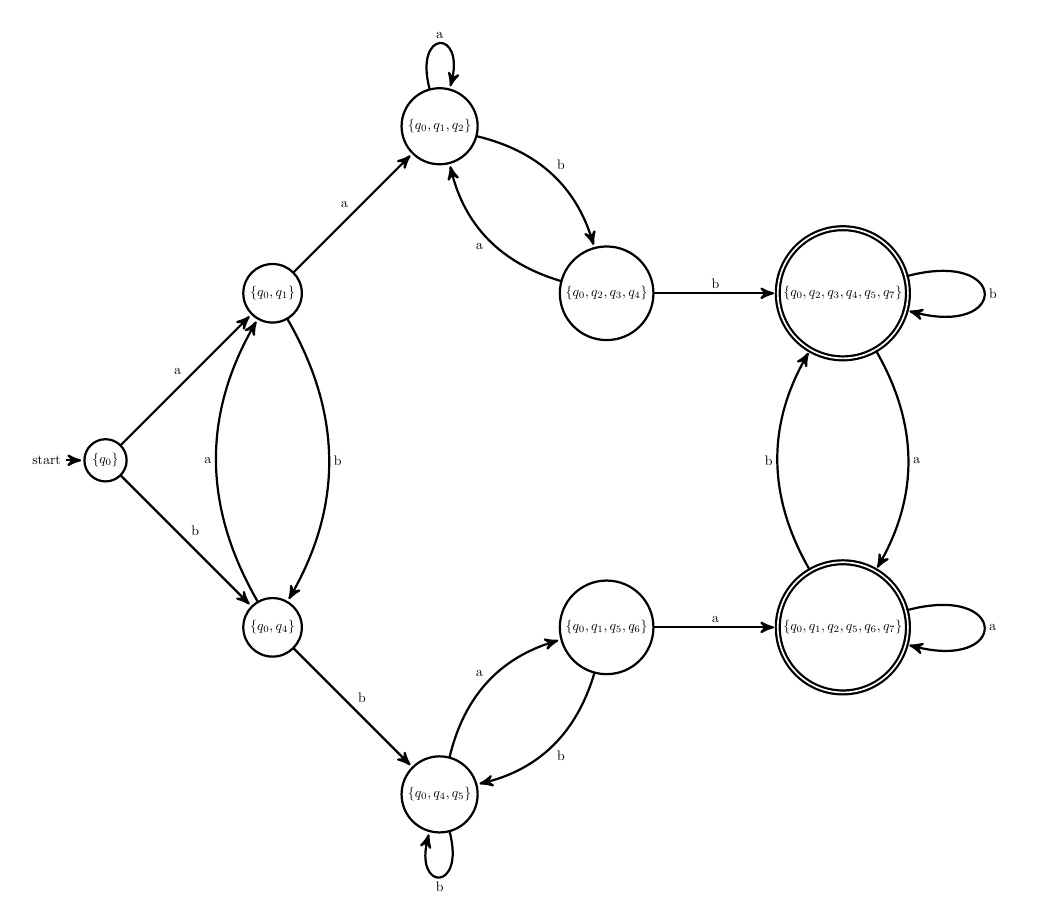
\begin{tikzpicture}[->,>=stealth',shorten >=1pt,auto,node distance=6cm,
                    thick, scale=0.5, every node/.style={scale=0.5}]
  \tikzstyle{every state}=[fill=white,draw=black,text=black]

  \node[initial,state] (q_0)                    {$\{q_0\}$};
  \node[state]         (q_0q_1) [above right of=q_0] {$\{q_0,q_1\}$};
  \node[state]         (q_0q_4) [below right of=q_0] {$\{q_0,q_4\}$};
  \node[state]         (q_0q_1q_2) [above right of=q_0q_1] {$\{q_0,q_1,q_2\}$};
  \node[state]         (q_0q_4q_5) [below right of=q_0q_4] {$\{q_0,q_4,q_5\}$};
  \node [state] (q_0q_2q_3q_4) [below right of=q_0q_1q_2] {$\{q_0,q_2,q_3,q_4\}$};
  \node [state] (q_0q_1q_5q_6) [above right of=q_0q_4q_5] {$\{q_0,q_1,q_5,q_6\}$};
  \node [state, accepting] (q_0q_2q_3q_4q_5q_7) [right of=q_0q_2q_3q_4] {$\{q_0,q_2,q_3,q_4,q_5,q_7\}$};
  \node [state, accepting] (q_0q_1q_2q_5q_6q_7) [right of=q_0q_1q_5q_6] {$\{q_0,q_1,q_2,q_5,q_6,q_7\}$};


  \path (q_0) edge              node {a} (q_0q_1)
                edge node {b} (q_0q_4)
        (q_0q_1) edge [bend left] node {b} (q_0q_4)
        edge node {a} (q_0q_1q_2)
        (q_0q_4) edge [bend left] node{a} (q_0q_1)
        edge node {b} (q_0q_4q_5)
        (q_0q_1q_2) edge [loop above] node {a} ()
        edge [bend left] node {b} (q_0q_2q_3q_4)
        (q_0q_4q_5) edge [loop below] node {b} ()
        edge [bend left] node {a} (q_0q_1q_5q_6)
        (q_0q_2q_3q_4) edge [bend left] node {a} (q_0q_1q_2)
        edge node {b} (q_0q_2q_3q_4q_5q_7)
        (q_0q_1q_5q_6) edge [bend left] node {b} (q_0q_4q_5)
        edge node {a} (q_0q_1q_2q_5q_6q_7)
        (q_0q_1q_2q_5q_6q_7) edge [loop right] node {a} ()
        edge [bend left] node {b} (q_0q_2q_3q_4q_5q_7)
        (q_0q_2q_3q_4q_5q_7) edge [loop right] node {b} ()
        edge [bend left] node {a} (q_0q_1q_2q_5q_6q_7)
        ;
\end{tikzpicture}
\newpage
\subsection*{d)}
\noindent
For NFA:\\
\begin{center}
\begin{forest}
  [\textit{$(q_0, bbabb)$}
    [\textit{$(q_0, babb)$}
        [\textit{$(q_0, abb)$}
            [\textit{$(q_0, bb)$}
                [\textit{$(q_0, b)$}
                    [\textit{$(q_0, e)$}]
                    [\textit{$(q_4, e)$}]
                ]
                [\textit{$(q_4, b)$}
                    [\textit{$(q_5, e)$}]
                ]
            ]
            [\textit{$(q_1, bb)$}]
        ]
        [\textit{$(q_4, abb)$}]
    ]
    [\textit{$(q_4, babb)$}
        [\textit{$(q_5, abb)$}
            [\textit{$(q_5, bb)$}
                [\textit{$(q_5, b)$}]
            ]
            [\textit{$(q_6, bb)$}]
        ]
    ]
  ]
\end{forest}
\end{center}

For each possible path through the NFA, we either reach empty string without otherside the accepting state or we reach a state that does not accept our current character. Therefore, $\omega '$ is not accepted by our NFA.\\\\
For DFA:\\
$(q_0, bbabb)\vdash(q_0q_4, babb)\vdash(q_0q_4q_5, abb)\vdash(q_0q_1q_5q_6, bb)\vdash(q_0q_4q_5, b)\vdash(q_0q_4q_5, e)$\\

Since we reached the empty string otherside the accepting state, we conclude that $\omega '$ is not accepted by our DFA.

\section*{Answer 2}
\subsection*{a)}
Complement of a regular language is another regular language by the closure properties\\

Theorem: Complement of an irregular language is an irregular language.\\

Proof: Let $A$ be an irregular language that does not obey the theorem. Then $\overline{A}$ is a regular language. Then, by the closure properties, $\overline{\overline{A}}$ is again, a regular language. But this contradicts with the first definition. Then we conclude, there is no irregular language of which its complement is a regular language.
\newpage
By combining and using the properties above, we can conclude that there is a biconditionality between the regularity of language $L_1$ and $L_2$. That is, $L_2$ is regular if and only if $L_1$ is regular and $L_2$ is irregular if and only if $L_1$ is irregular.\\\\
Assume that $L_1$ is regular.\\
Let $l$ be the pumping length.\\
There is a split $w = xyz$ for all $|w|\geq l$, $|xy|\leq l$, $y\neq e$ and $xy^iz\in L_1$.\\
For even l: p = $l$\\
For odd l: p = $l+1$\\\\
$w = a\textsuperscript{p/2+1}b\textsuperscript{p/2}$\\
First possible split: x=$a^{p/2+1}$ , y=$b^{s}$, z=$b^{p/2-s}$ (s $\leq$ p/2 - 1)\\
For i $\geq$ 3, $xy^iz$ is not in the language. This split is not valid.\\
Second possible split: x=$a^{p/2+1-t}$ , y=$a^{t}b^{s}$, z=$b^{p/2-s}$ (s $\leq$ p/2 - 1)\\
For i $>$ 1, $xy^iz$ is not in the language. This split is not valid.\\
Third possible split: x=$a^{p/2+1-t}$ , y=$a^{t}$, z=$b^{p/2}$\\
For i = 0, $xy^iz$ is not in the language. This split is not valid.\\\\

Since no split can satisfy the pumping lemma conditions, $L_1$ is not regular. By the theorems above, neither $L_2$ is regular.
\subsection*{b)}
\noindent
Proof that $L_5$ is regular:

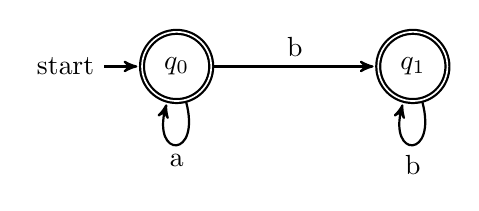
\begin{tikzpicture}[->,>=stealth',shorten >=1pt,auto,node distance=3cm,
                    thick]
  \tikzstyle{every state}=[fill=white,draw=black,text=black]

  \node[initial,state,accepting] (q_0)                    {$q_0$};
  \node[state,accepting] (q_1)      [right of=q_0]                      {$q_1$};

  \path (q_0) edge          [loop below]    node {a} (q_0)
        edge node {b} (q_1)
        (q_1) edge [loop below] node {b} (q_1)
        ;
\end{tikzpicture}

Since a NFA can be drawn for $L_5$, $L_5$ is regular.\\\\
Proof that $L_6$ is regular:

Since $L_6$ can be expressed by a regular expression $L_6$ is regular.\\\\

$L_4\cup L_5\cup L_6 = L_5\cup L_6$ since $L_4$ is a subset of $L_5$. (In $L_5$'s definition, if we choose m = n $\neq$ 0 we reach $L_4$). Thus, $L_4\cup L_5 = L_5$\\\\
$L_5\cup L_6$ is regular since $L_5$ and $L_6$ are both regular. (by the closure properties)

\end{document}